\documentclass{scrreprt}
\usepackage{graphicx}
\usepackage[utf8]{inputenc}
\usepackage{tikz}
\usepackage{listings}
\usepackage{underscore}
\usepackage[bookmarks=true]{hyperref}
\usepackage{placeins}
\usepackage{caption}
\hypersetup{
    bookmarks=false,    % show bookmarks bar?
    pdftitle={Software Requirement Specification},    % title
    pdfauthor={Yiannis Lazarides},                     % author
    pdfsubject={TeX and LaTeX},                        % subject of the document
    pdfkeywords={TeX, LaTeX, graphics, images}, % list of keywords
    colorlinks=true,       % false: boxed links; true: colored links
    linkcolor=blue,       % color of internal links
    citecolor=black,       % color of links to bibliography
    filecolor=black,        % color of file links
    urlcolor=purple,        % color of external links
    linktoc=page            % only page is linked
}%
\def\myversion{1.0}
\date{}
\usepackage{hyperref}
\begin{document}
\begin{titlepage}
  \flushright\bfseries\huge
  \vspace*{\stretch{0.4}}
    \rule{\linewidth}{5pt}
    \par
    \vspace{1cm}
    {\Huge DESIGN \par DOCUMENT \par}
    \vspace{2cm}
    for \\
    \vspace{2cm}
    Personal Dietary Application \\
    \vspace{2cm}
     \LARGE{Version \myversion \\}
    \vspace{2cm}
    by Craig Boucher \\
    Md Tanveer Alamgir \\
    Fan \\
    Osman \\
    Xin
    \vspace{2cm}
    \rule{\linewidth}{5pt}
    \vspace{\stretch{1}}
\end{titlepage}
\tableofcontents
\chapter{Introduction}
The project undertaken in this COMP 5541 course involves creating an application that keeps track of dietary records for the user. This diet app has been designed to use the border pane layout for the main window. \\ \\ 
This design document will provide details for the type of software architecture used to develop the software and explain the design for the user interface. The architectural component illustrates the abstraction of the software classes involved and how they relate to each other to maniuplate and process data that the user interacts with. The interface design section will assess the process for the states the user goes through to interact with the personal dietary application.
\section{Purpose}
This document will serve as an illustration for the architectural design choices as well as an explanation for the properties of the user interface implemented for the Personal Dietary Application software. This software project is being completed for the COMP 5541 graduate diploma course at Concordia University. There will be diagrams to chowcase the type of the architecture used and a class diagram. Screenshots are used to provide a valuable perspective on the user interface. These graphical aids are described in further detail to demonstrate the functionality of the interface.
\section{Scope}
In order to provide proper design documentation for the Personal Dietary Application this document will be properly formatted and included all necessary information. The team responsible for surveying this document and creating the software will be able to use the robust explanation of the architectural model presented in this document to carry out the necessary work. The visual graphics demonstrating the user interface design choices will serve as a guide for the team to orchestrate the proper performance of the software.
\section{Definitions and Abbreviations}
\subsection{Definitions}
\begin{tabular}{|l|l|}
\hline
	Term & Definition \\
\hline
	Model View & Software architecture that renders funcionality between three components. \\
	Controller & The view is the user interface. The model stores the data and the controller \\
	& mediates data transfer between the view and model. \\
\hline
	Date & Allows user to enter day and month of an entry for an item. \\
\hline
	Consumed & The user will be able to mark a food item as consumed (eaten) or not. \\
\hline
\end{tabular}

\subsection{Abbreviations}
\begin{tabular}{|l|l|}
\hline
	Abbreviation & Term \\
\hline
	MVC & Model View Controller \\
\hline
	GUI & Graphical User Interface \\
\hline
	UML & Unified Modeling Language \\
\hline
	PDA & Personal Dietary Application \\
\hline
\end{tabular}

\section{References}
https://upload.wikimedia.org/wikipedia/commons/a/a0/MVC-Process.svg \\
http://users.encs.concordia.ca/~paquet/wiki/images/e/ee/Phase2final.pdf
\section{Overview}
The rest of the document is composed of two main sections. First, there is a section dedication to Architectural Design. Lastly, the largest section, consists of Software Interface Design. In the portion concerning the software architecture the three smaller sections are related to the reasoning for choosing the architecture, a diagram illustrating how the architecture behaves abstractly, and the final section details how software files will operate together on the computer. \\
The interface section will provide documentation regarding the system, modules, and dynamic interfaces for the software project.
\chapter{Architectural Design}
\section{Rationale}
The Model View Controller (MVC) architecture design pattern has been chosen for this software project. Model, View, and Controller are the three components which comprise this architecture. \\

The purpose of the Controller model is to navigate and facilitate the transfer of data between the View and the Model. The Controller is responsible for acquiring data input from the user, manipulate the model with the necessary memory changes, and potentially provide updates to the View if and when exceptions or errors are thrown. \\

The View is where the (graphical) user interface rests. The information stored in the model is used by the View to display everything necessary to the user. Everything the user interacts with rests with the View, from input functionality to button objects. Whenever data is manipulated in the Model the View will reflect this accordingly. \\

The objective of the Model is to store all of the necessary information and data that the application requires to operate successfully. All of the data is stored in local memory. Every food item and all of the details of each item is stored in the Model module. There is a list of every food item added by the user that is stored in the Model, and whenever a change is made (adding or removing food items), the View will graphically respond to these changes. \\

\begin{center}
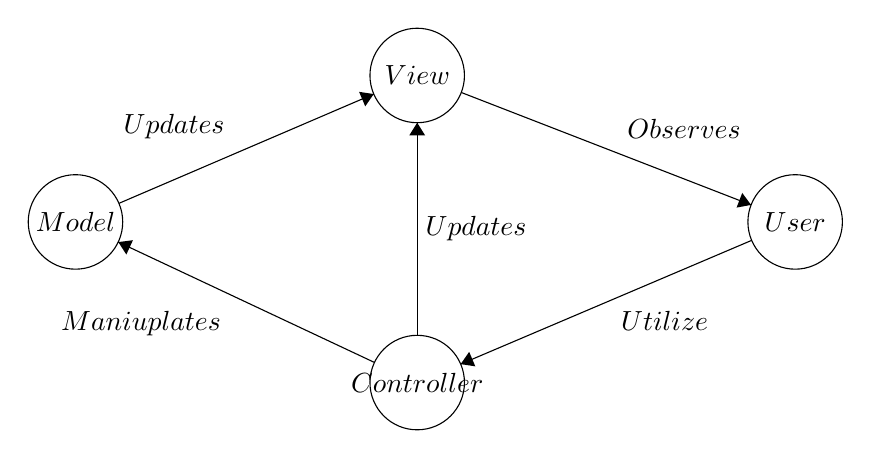
\begin{tikzpicture}[scale=0.2]
\tikzstyle{every node}+=[inner sep=0pt]
\draw [black] (39.5,-15.1) circle (3);
\draw (39.5,-15.1) node {$View$};
\draw [black] (17.8,-24.4) circle (3);
\draw (17.8,-24.4) node {$Model$};
\draw [black] (39.5,-34.6) circle (3);
\draw (39.5,-34.6) node {$Controller$};
\draw [black] (63.5,-24.4) circle (3);
\draw (63.5,-24.4) node {$User$};
\draw [black] (42.3,-16.18) -- (60.7,-23.32);
\fill [black] (60.7,-23.32) -- (60.14,-22.56) -- (59.78,-23.49);
\draw (56.44,-19.14) node [above] {$Observes$};
\draw [black] (60.74,-25.57) -- (42.26,-33.43);
\fill [black] (42.26,-33.43) -- (43.19,-33.57) -- (42.8,-32.65);
\draw (55.21,-30.05) node [below] {$Utilize$};
\draw [black] (36.78,-33.32) -- (20.52,-25.68);
\fill [black] (20.52,-25.68) -- (21.03,-26.47) -- (21.45,-25.56);
\draw (21.96,-30.05) node [below] {$Maniuplates$};
\draw [black] (20.56,-23.22) -- (36.74,-16.28);
\fill [black] (36.74,-16.28) -- (35.81,-16.14) -- (36.2,-17.06);
\draw (24.06,-19.19) node [above] {$Updates$};
\draw [black] (39.5,-31.6) -- (39.5,-18.1);
\fill [black] (39.5,-18.1) -- (39,-18.9) -- (40,-18.9);
\draw (40,-24.85) node [right] {$Updates$};
\end{tikzpicture}
\end{center}

The software specifications outlined in the project instructions specifically mandated the MVC architecture. The purpose of this architecture is to provide a relevant abstraction of how desktop, mobile, or web applications operate when requiring constant use by a user. The abstraction allows three distinct modules to operate independently of each other and be capable of being updated separately. Different developers can be assigned to develop for the various modules with minimal cooperation required between them as the core functionality of each module remains the same across updates.

\section{Software Architecture Diagram}
\includegraphics[height=9cm]{MVC-Process.png}
\section{System Topology}
\chapter{Software Interface Design}
\section{System Interface Diagrams}

Our personal dietary application has only system level interface. The application does not employ any software or hardware interfaces. GUI is the system level interface. GUI allows the user to interact with the application. Using GUI user will be able to add a food item, mark it as eaten or not eaten, hide an added item, remove an item and the update of the dietary.

\subsection{User Interface}

User will interact with the computer using the user interface. We tried to make it as user friendly as possible by placing the components with an order of their importance and utilizing the full screen mode. Below are the few points we took into consideration for user interface:

\begin{itemize}
\item User Friendly: Making it user friendly by putting important components according to user's view point.
\item Easy to find information: Since the application is all about their dietary, so it was important to make it easy to calculate and display their consumed and need to consumed items. We make it as handy as possible.
\item Guiding user: Guiding user by displaying different colour if they miss out something while inputting a food item.
\end{itemize}

\section{Dynamic Models of System Interface}
The system interfaces that establish the interaction between user and computer are described below:

\clearpage

\subsection{Landing page}
Below is the first screen user will see when they will launch the application. Here is the description of every options available to user:

\begin{figure}[!htbp]
\centering
\includegraphics[width=15cm]{pictures/raw.png}
\caption*{Landing page}
\end{figure}
\FloatBarrier
\begin{enumerate}
\item Add a food item: User can input the food details to have it added.
\item Display the added food: It's a list of all food added by user
\item Remove a food item: It's a button to remove a food item from added list.
\item Hide/unhide Consumed food: This button gives the user ability to hide/unhide consumed food.
\item Total serving: It will show the total serving of all the items in the added food list.
\item Serving of consumed item: This will only show the total serving of consumed item(s).
\item Food group: Based on the food item(s) added and consumed these 4 button will indicate which group they belong to.
\end{enumerate}
	
\subsection{Add Food Item Scenario}

Below gives the ability to an user to add a food item by inserting the details of the food:

\begin{figure}[!htbp]
\centering
\includegraphics[width=15cm]{pictures/add-food-item.png}
\caption*{Add a food item}
\end{figure}

\FloatBarrier

\begin{enumerate}
\item Name: User will insert the name of the food.
\item Date: User will select the date from the calendar on the right side of the text box.
\item Time: User will insert the time of the food consumed. Time the is in 24h formate.
\item Food Group: User will select the respective food group from the drop down menu.
\item Meal: User will insert the meal they consumed the food at.
\item Type: This field is for user to indicate whether the food was bought, homemade. If the food was consumed at out dining then this field will get greyed out.
\item Retailer: This is to identify the name of the retailer if the food was consumed from out dining. If in dining is selected using the toggle switch at the bottom then this field will be greyed out.
\item Amount: The amount of food consumed by the user.
\item Calories: The amount of calories presented in the consumed food.
\item Fat: The amount of fat presented in the consumed food.
\item Sodium: The amount of Sodium presented in the consumed food.
\item Sugar: The amount of Sugar presented in the consumed food.
\item Toggle Switch (In dining/Out Dining): This toggle switch will allow the user to choose whether the food was consumed inside of outside.
\item Add Item: After Filling out all the details of the food user will press the Add Item button to add the food item.
\item Validation: If user does not fill out all the fields then the placeholder will show up to indicate which field needs to be filled out and what to put inside that field

\begin{figure}[!htbp]
\centering
\includegraphics[width=5cm]{pictures/err-add-item.png}
\caption*{Validation of input}
\end{figure}

\FloatBarrier
\end{enumerate}

Once a food item has been added successfully the details will show up on the list section at the middle of the page. As we keep on adding food items on the very left side the total serving will be calculated. This serving is not for consumed item(s), this is the total of all the food items added by user.
\pagebreak
\subsection{Set Food Item as Consumed Scenario}

\begin{figure}[!htbp]
\centering
\includegraphics[width=15cm]{pictures/consumed.png}
\caption*{Mark as consumed}
\end{figure}

\FloatBarrier

In the display list of the food item(s) user will have the option to mark a food as consumed by clicking the checkbox in "Consumed" column. As user keeps on marking different food items as consumed from display list the total serving (Total serving of consumed list) will be changing on the left side.

\subsection{Set Food Item as Unconsumed Scenario}

If a food has been marked as consumed, user has the option to click on the checkbox again of the same food to remove the mark and make it as unconsumed. After making a food unconsumed the serving of that particular food will be deducted from the "Total serving of consumed food".

\subsection{Remove Food Item Scenario}

\begin{figure}[!htbp]
\centering
\includegraphics[width=15cm]{pictures/remove-food.png}
\caption*{Remove a food item}
\end{figure}

\FloatBarrier

To remove a food item there are two steps user needs to follow:

\begin{enumerate}
\item Step 1: First user needs to select the item he/she wants to remove from the display list.
\item Step 2: Then he/she needs to click the remove button.
\end{enumerate}

\subsection{Hide Consumed Diet Scenario}

\begin{figure}[!htbp]
\centering
\includegraphics[width=15cm]{pictures/hide.png}
\caption*{Hide consumed item(s)}
\end{figure}

\FloatBarrier

When user clicks the "Hide/Unhide Consumed" button on the right had side all the consumed food item(s) will disappear from the display list. It also update the "Total serving of displayed items" as this list display the serving of all displayed food items.

\subsection{Unhide Consumed Diet Scenario}

When all the item(s) are hidden by a user then user can click the same "Hide/Unhide Consumed" button again to make all the consumed food item(s) appear on the display list. Also "Total serving of displayed items" list will be updated.

\pagebreak

\subsection{Marking food Group}

\begin{figure}[!htbp]
\centering
\includegraphics[width=15cm]{pictures/food-group.png}
\caption*{Marking good group}
\end{figure}

\FloatBarrier

To mark a food group user does not need to do anything explicitly. During the adding of a food item they need to select a food group from drop down. Once a food group has been selected and added in the display list the respective food group will light up in green colour. On the other hand if user removes a food item from the display list and there is no food item present of a particular food group in the display list then that food group will set back to grey colour indicating there is no food present in the list of that food group.

\section{Module Interface Diagrams}

\begin{center}
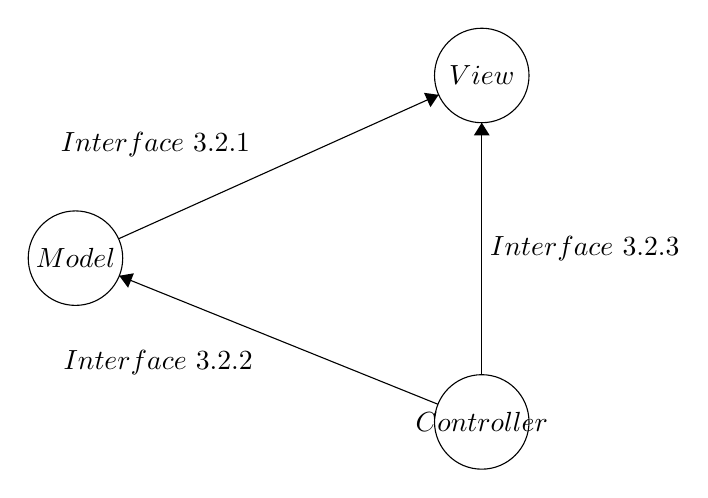
\begin{tikzpicture}[scale=0.2]
\tikzstyle{every node}+=[inner sep=0pt]
\draw [black] (39.5,-15.1) circle (3);
\draw (39.5,-15.1) node {$View$};
\draw [black] (13.7,-26.7) circle (3);
\draw (13.7,-26.7) node {$Model$};
\draw [black] (39.5,-37.1) circle (3);
\draw (39.5,-37.1) node {$Controller$};
\draw [black] (36.72,-35.98) -- (16.48,-27.82);
\fill [black] (16.48,-27.82) -- (17.04,-28.58) -- (17.41,-27.66);
\draw (18.95,-32.54) node [below] {$Interface\mbox{ }3.2.2$};
\draw [black] (16.44,-25.47) -- (36.76,-16.33);
\fill [black] (36.76,-16.33) -- (35.83,-16.2) -- (36.24,-17.11);
\draw (18.78,-20.32) node [above] {$Interface\mbox{ }3.2.1$};
\draw [black] (39.5,-34.1) -- (39.5,-18.1);
\fill [black] (39.5,-18.1) -- (39,-18.9) -- (40,-18.9);
\draw (40,-26.1) node [right] {$Interface\mbox{ }3.2.3$};
\end{tikzpicture}
\end{center}

\subsection{View Interface}

This is the View part of MVC (Model View Controller) design pattern. It holds all the classes that together build GUI of our application. Following are the classes and methods of all the classed inside view:

\subsubsection{FXApp}

It holds the main method of our application. Since we are using JAVAFx so we are initializing the BorderPane, Scene, Stage and then call the show method to run the application.

\subsubsection{FXController}

In this class we initialized the Left, Right, Center and Bottom part of the border pane. Below are the methods this class contains:

\begin{itemize}
	\item initialize(): It calls the four methods whenever a user opens the application. The four different methods are: initialLeftPart(), initialRightPart(), initialBottomPart(), initialCenterPart().
	\item initialCenterPart(): This is a table where the added food item gets listed. Every time user adds a food item the table gets updated.
	\item initialLeftPart(): The form to add a food item lyes here. We used grid pane to organize the form on the left side of the border pane. It also contains an event handler named addEventHandler. Here we distinguish the in dining and out dining serving. This 				handler also updates the data in the model of MVC so the list food display list always gets updated. Whenever user press the "Add Item" this handler gets triggered and update the display list in the centre and serving on the left side of the GUI.
	\item initialRightPart(): Items here are organized using grid pane. It has remove, Hide/Unhide Buttons and the list of "Total serving of Displayed item" and "Total serving of consumed items". Upon clicking the "Remove button" it does below things:
	\begin{itemize}
		\item Make sure the display list is not empty.
		\item Remove the selected food item from the table (Display table)
		\item Update the food group. If the removed item was the last item of that food group the set the colour of that food group to grey.
		\item Update the total serving of displayed items.
		\item Update the total serving of consumed items.
	\end{itemize}
	Upon clicking the "Hide/Unhide Consumed items" button:
	\begin{itemize}
		\item Check if the consumed items are already hidden. If so then update the diningManager to unhide them.
		\item If consumed items are not hidden then update the diningManager to hide consumed items.
		\item For each of the above change it will update the list of "Total serving of consumed items".
	\end{itemize}
	\item initialBottomPart(): We used HBox of JavaFx to organize the four buttons that updates food group.
	\item refreshItems(): Once user add a food item by clicking the "Add Item" button this method clears out all the fields in for form on the left side of the GUI.
	\item stringToGroup(): Return the type of FoodGroup by the name of the food group selected by user.
	\item markFoodGroupAdd(): There are four different counters for one for each Food Group to keep track how many food items belong to an individual group. This method increases that counter for an individual food group and sets the background colour green 				once a food has been added for a particular food group.
	\item markFoodGroupRemove(): It decreases the counter for a food group and sets the colour grey if there is no food listed in the display table.
\end{itemize}

\subsubsection{DiningTableRow}
\subsection{Model Interface}
\subsection{Controller Interface}

% add other chapters and sections to suit
\end{document}
